\chapter{The CMS experiment}
\label{chap:cms}
\chapterquote{I'm a bus}
{Darren Burton 1987--2013}

\section{Description}

Brief description of the LHC. Description of the CMS detector with particular focus the ECAL .

\textbf{15 pages}

The \acf{lhc} is a big particle accelerator.
One of the experiments there is called \acf{cms} which contains an \acf{ecal} and a \acf{hcal}. Sometimes we use \acf{bdts} which are a type of \acf{mva}.

\begin{figure}
  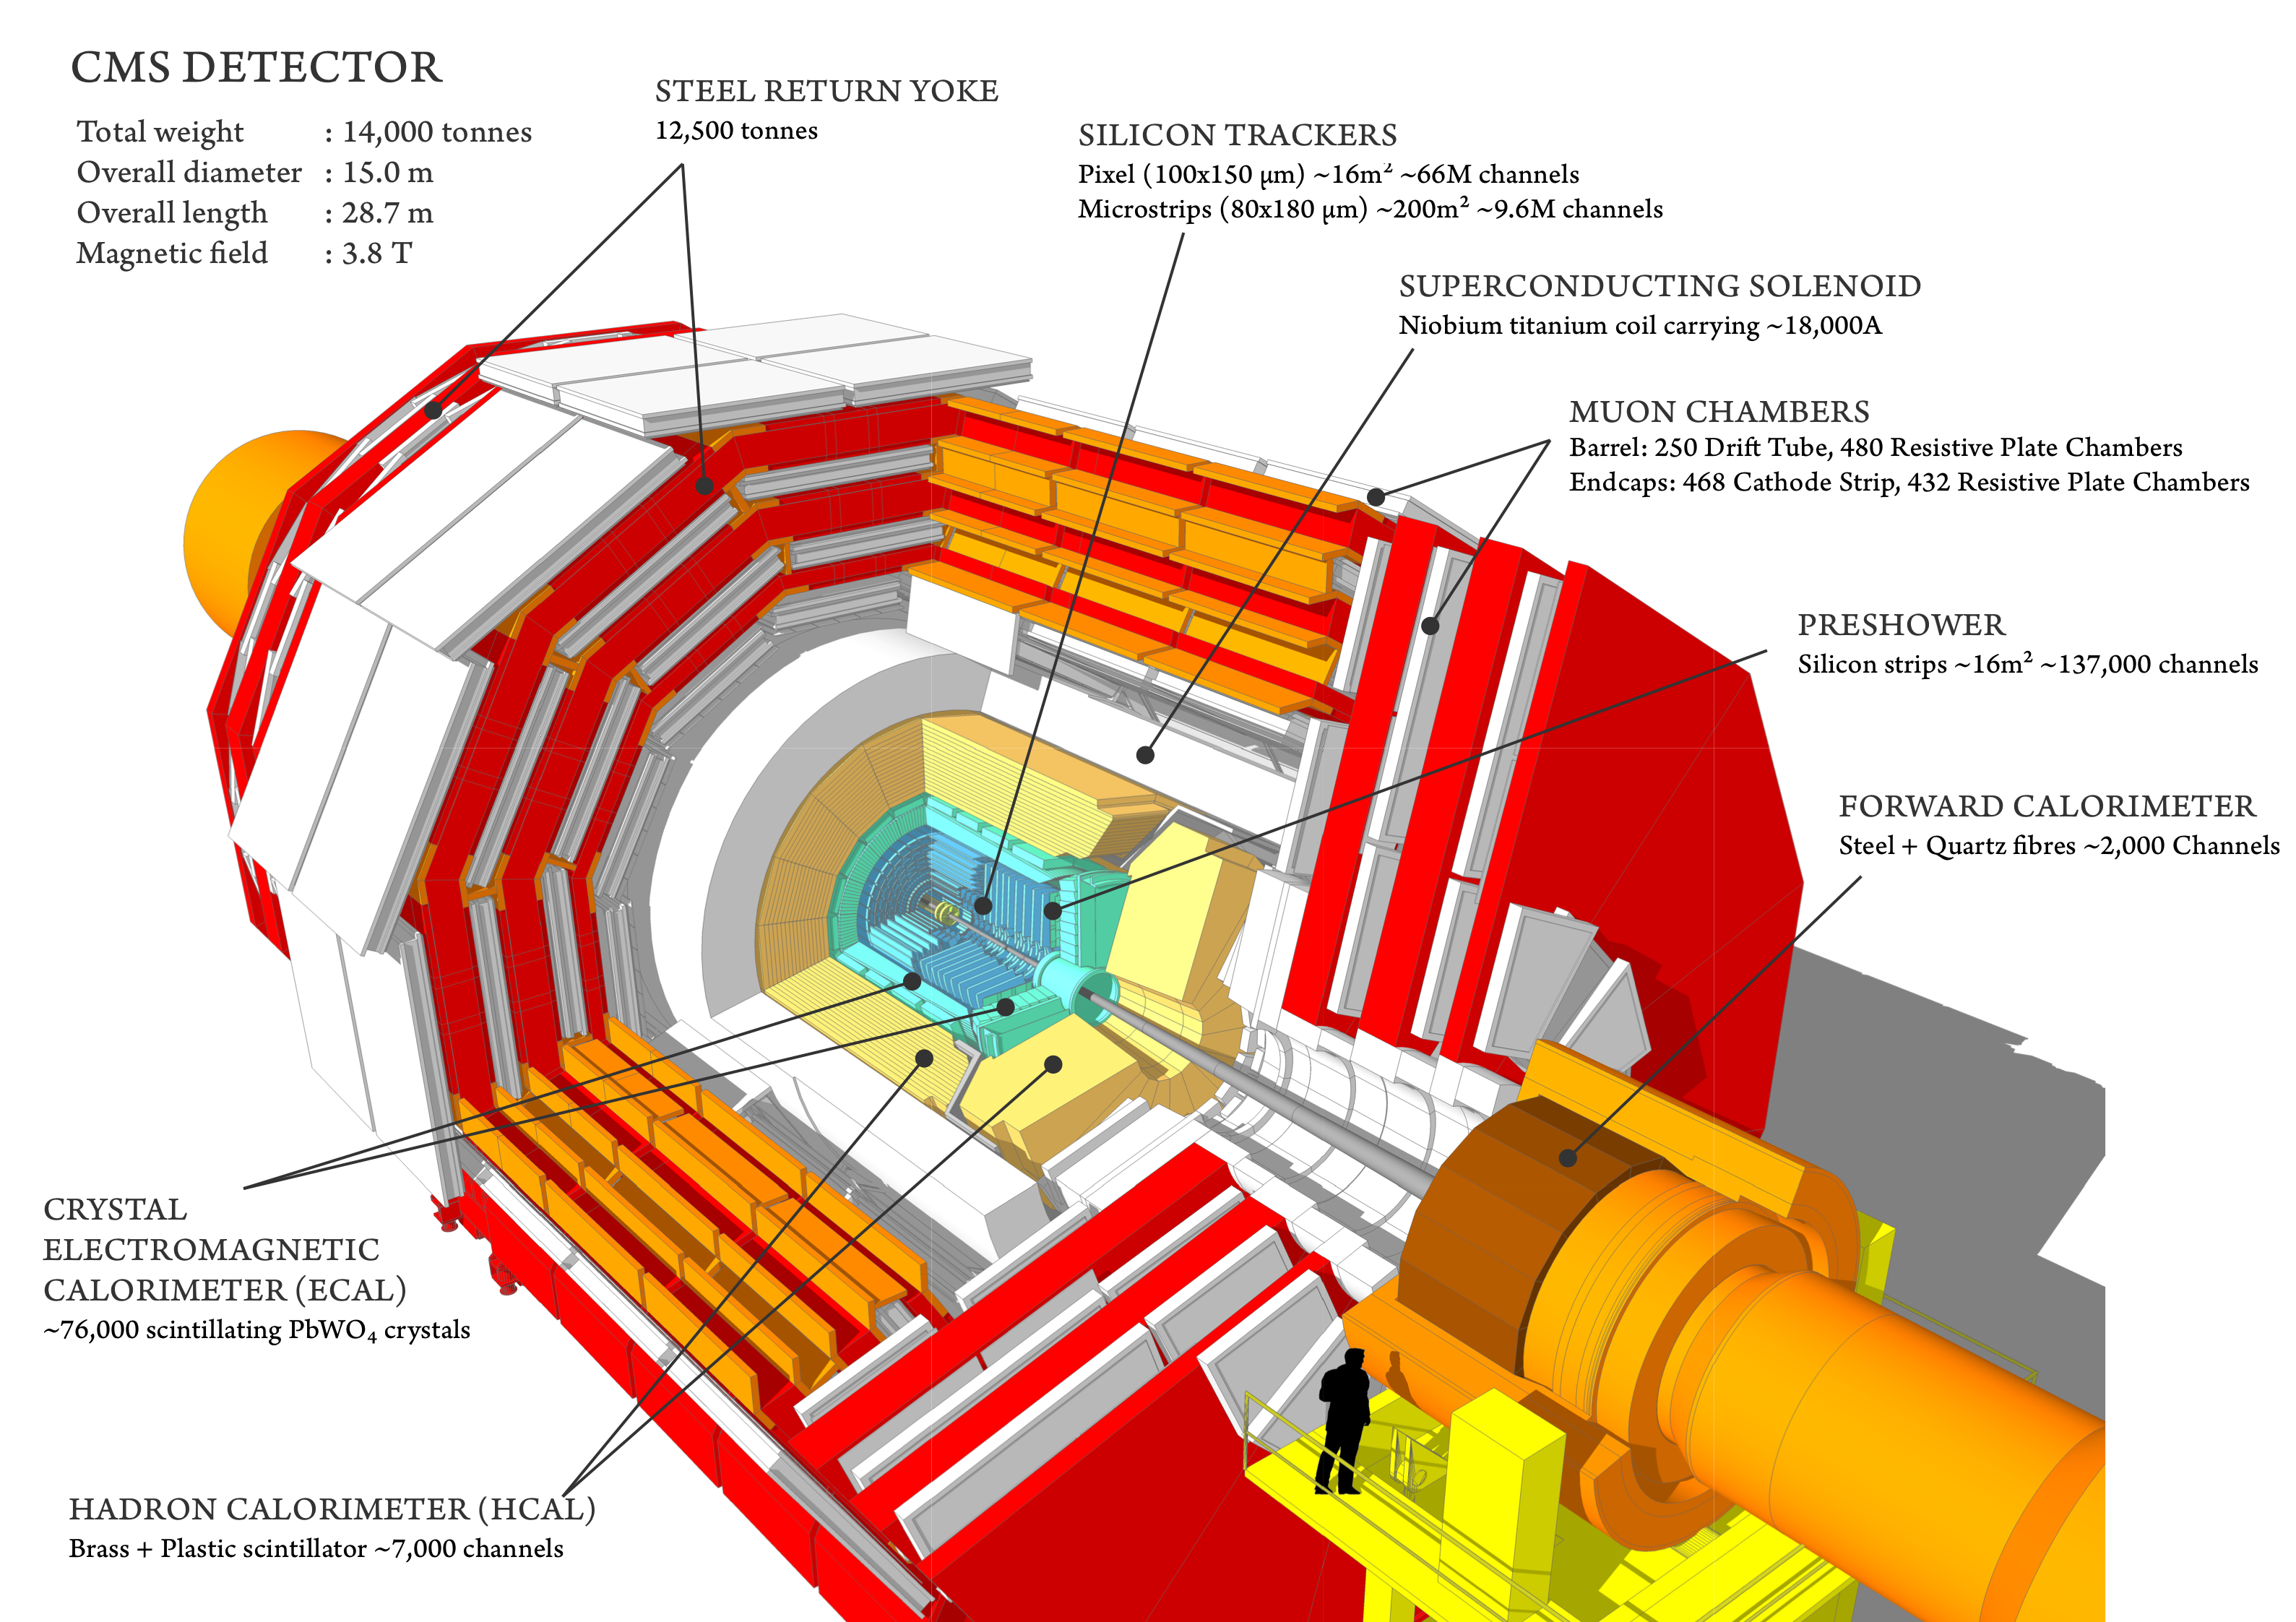
\includegraphics[width=0.8\textwidth]{ch2_cms_exp/plots/cms_diagram.png}
  \caption[CMS diagram]{This is a schematic representation of \ac{cms}}
  \label{fig:cms_diagram}
\end{figure}
